This paper investigates the decoding performance of convolutional codes. This is done by simulating end-to-end transmission in different channels where messages are encoded using various convolutional codes.
Figure \ref{fig:simulationOverview} shows the logical setup of the simulation.

\begin{figure} [h]
\usetikzlibrary{shapes,arrows}

\tikzstyle{block} = [draw, rectangle, minimum height=3em, minimum width=6em]
\tikzstyle{input} = [coordinate]
\tikzstyle{output} = [coordinate]

\centering
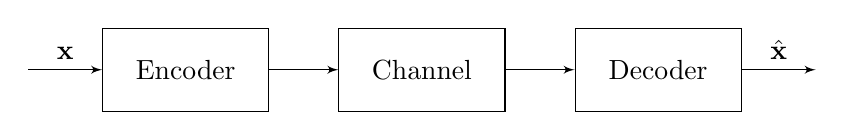
\begin{tikzpicture}[auto, node distance=2cm,>=latex']
\centering

    % We start by placing the blocks
    \node [input, name=input] {};    
    \node [block, right of=input] (encoder) {Encoder};
    \node [block, right of=encoder, node distance=3cm] (channel){Channel};
    \node [block, right of=channel, node distance=3cm] (decoder){Decoder};
    \node [output, right of=decoder] (output) {}; 
    
    
    \draw [->] (encoder) -- node[name=u] {} (channel);
    \draw [->] (channel) -- node[name=v] {} (decoder);
    \draw [draw,->] (input) -- node {$\textbf{x}$} (encoder);
    \draw [->] (decoder) -- node [name=y] {$\hat{\textbf{x}}$}(output);

\end{tikzpicture}
\caption{\textit{Simulation overview} \label{fig:simulationOverview}}
\end{figure}

A message, $\textbf{x}$, consisting of $10^6$ bits is sent over a noisy channel. 2 types of channels are considered in this study:
\begin{itemize}\setlength\itemsep{0pt}
   \item Binary Symmetric Channel (BSC): Random, independant errors occur during transmission. The typical representation of a binary symmetric channel is shown in figure \ref{fig:bscChannel}
   \item Burst Error Channel: Errors are not independant, but occur in bursts.
\end{itemize}

\begin{figure} [b]
\centering
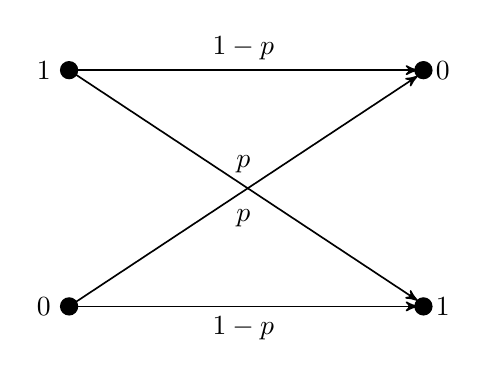
\begin{tikzpicture}[->, >=stealth', auto, semithick, node distance=3cm]
\centering
\filldraw (0,0) circle (3pt);
\filldraw (0,3) circle (3pt);
\filldraw (4.5,0) circle (3pt);
\filldraw (4.5,3) circle (3pt);
\draw[->,line width=0.6pt] (0,3) node[left=3pt] {$1$} -- node[above=1pt] {$p$} (4.425,0.075);
\draw[->,line width=0.6pt] (0,0) node[left=3pt] {$0$} -- node[below=3pt] {$p$} (4.425,2.925);
\draw[->,line width=0.6pt] (0,0) -- node[below] {$1-p$} (4.425,0.00)  node[right=3pt] {$1$};
\draw[->,line width=0.6pt] (0,3) -- node[above] {$1-p$} (4.425,3) node[right=3pt] {$0$};
\end{tikzpicture}
\caption{\textit{Binary Symmetric Channel}\label{fig:bscChannel}}
\end{figure}

The purpose of the study is to quantify the effects of different parameters of the convolutional code, namely the constraint length and the code rate. In order to achieve the best performance a trade-off analysis on the parameters needs to be performed. 
All simulations are conducted by utilizing MATLAB. Section \ref{sec:methodSection} presents the approach used to systematically determine the effect of code parameters in different channels. \todo{Analysis performed in sections 2-3-4}. Finally, section \ref{sec:conclusionSection} summarizes the findings.

